\documentclass[aspectratio=169]{beamer}
\setbeamertemplate{navigation symbols}{}
\usepackage{color,amsmath,comment, subfigure}
\usepackage{booktabs}
\usepackage{url}

%%%%%%%%%%%%%%%%%%%%%%%%%%
\title[]{The connected age and the small world problem}
\author[]{Social Networks (Soc 204)\\Spring 2021\\Princeton University}
\institute[]{Matthew J. Salganik}
\date[]{Week 1, Lecture 2\\ Video 3/3: Small world extension

\vfill

\begin{flushleft}
\vspace{0.7in}

\includegraphics[width=0.05\textwidth]{figures/cc.png}
\end{flushleft}

}

\begin{document}
%%%%%%%%%%%%%%%%%%%%%%%%%%%
\frame{\titlepage}
%%%%%%%%%%%%%%%%%%%%%%%%%%
\begin{frame}

\begin{center}
\includegraphics<1>[height=0.8\textheight]{figures/1967_Ford_Fairlane_Ranchero.jpg}
\end{center}

\vfill
\tiny{\url{http://upload.wikimedia.org/wikipedia/commons/f/f5/1967_Ford_Fairlane_Ranchero.jpg}}

\end{frame}
%%%%%%%%%%%%%%%%%%%%%%%%%%%
\begin{frame}

\begin{center}
\includegraphics<1>[height=0.8\textheight]{figures/Ericsson_Dialog_in_green}
\end{center}

\vfill
\tiny{\url{http://commons.wikimedia.org/wiki/File:Ericsson_Dialog_in_green.JPG}}

\end{frame}
%%%%%%%%%%%%%%%%%%%%%%%%%%%
\begin{frame}

\begin{center}
\includegraphics<1>[height=0.8\textheight]{figures/Computer_in_County_of_Orange_offices,_1967}
\end{center}

\vfill
\tiny{\url{http://commons.wikimedia.org/wiki/File:Computer_in_County_of_Orange_offices,_1967.jpg}}

\end{frame}
%%%%%%%%%%%%%%%%%%%%%%%%%%%
\begin{frame}

\begin{center}
\includegraphics<1>[height=0.8\textheight]{figures/detriot_race_riot_1967}
\end{center}

\vfill
\tiny{\url{http://content.time.com/time/covers/0,16641,19670804,00.html}}\\
Detroit 12th street riots: more than 40 people died, more than 1,000 injured, and more than 2,000 buildings destroyed

\end{frame}
%%%%%%%%%%%%%%%%%%%%%%%%%%%
\begin{frame}

\begin{center}
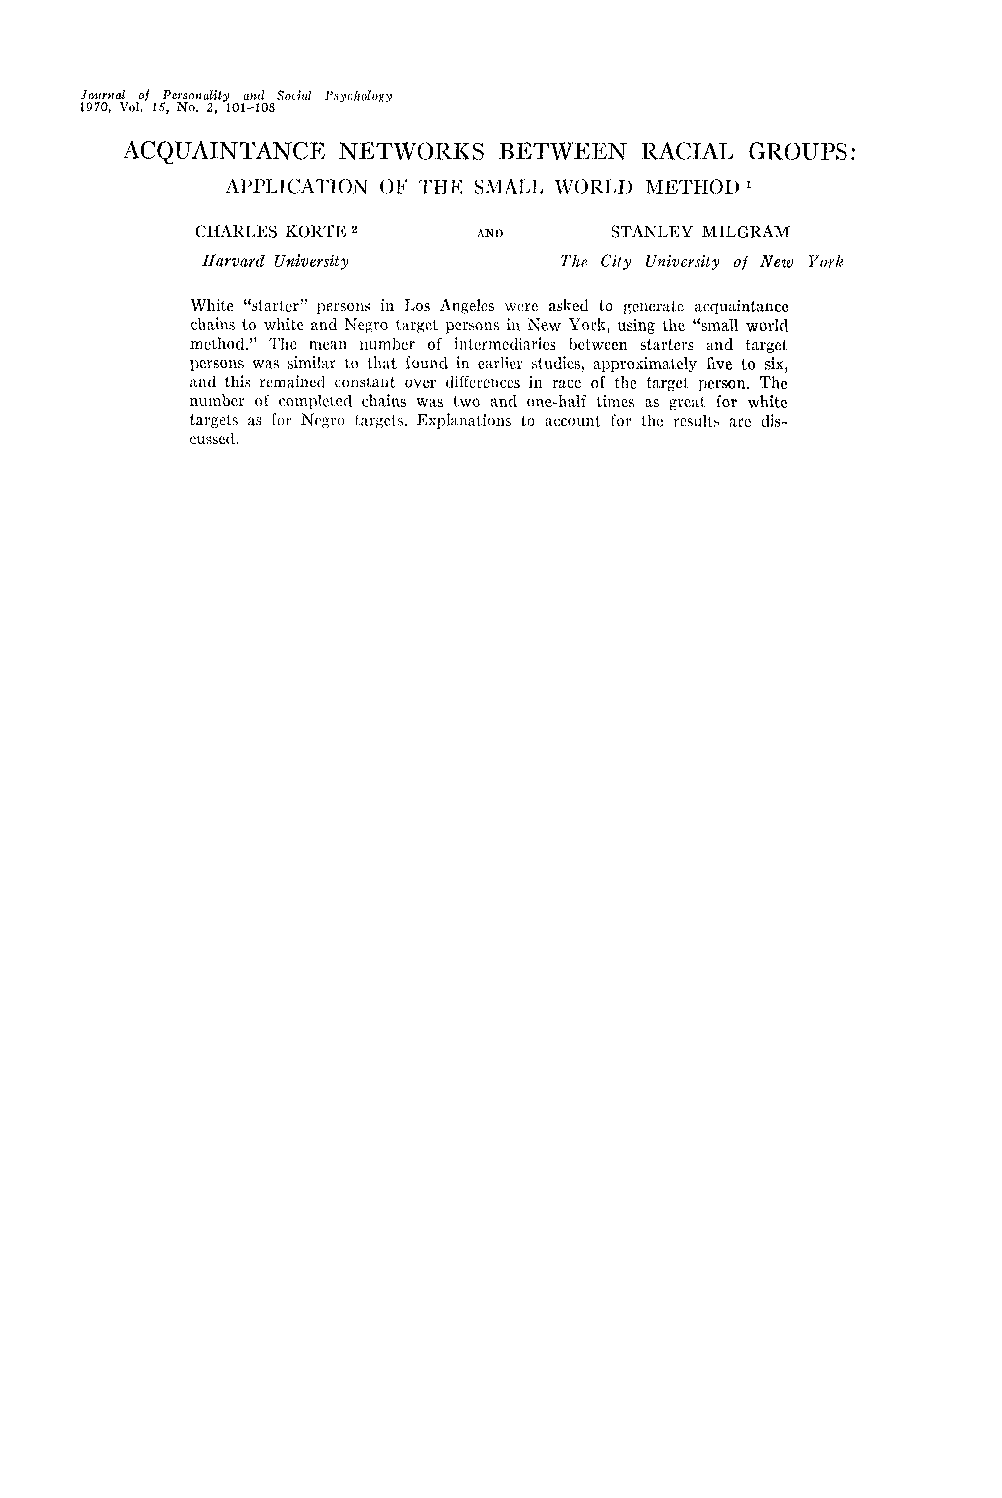
\includegraphics[width=0.9\textwidth]{figures/korte_aquaintance_1970_title}
\end{center}

\vfill
\url{http://dx.doi.org/10.1037/h0029198}

\end{frame}
%%%%%%%%%%%%%%%%%%%%%%%%%
\begin{frame}

540 white starters in LA\\
\pause

18 targets:
\begin{center}
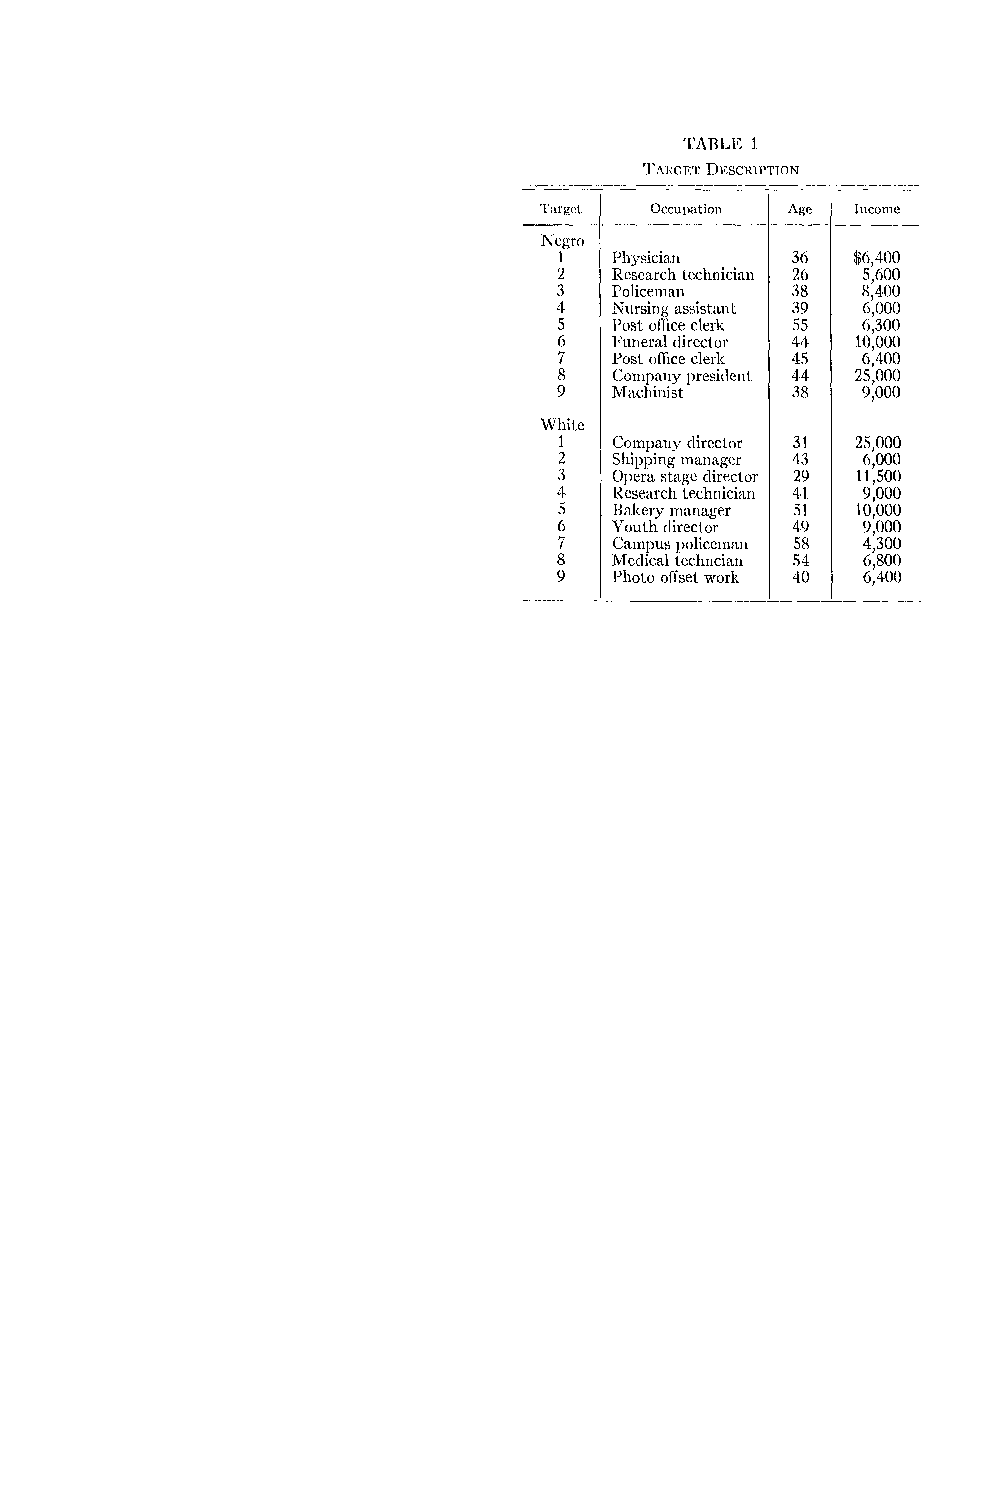
\includegraphics[height=0.6\textheight]{figures/korte_aquaintance_1970_tab1}
\end{center}

\vfill
Race of target was not explicitly known to participants

\note{
Note how Milgram spends his complexity, doesn't vary starter location any more, chooses to vary something else
}

\end{frame}
%%%%%%%%%%%%%%%%%%%%%%%%%
\begin{frame}
\frametitle{Result 1}

\begin{center}
\includegraphics<1>[height=0.8\textheight]{figures/korte_aquaintance_1970_fig1}
\end{center}

Mean intermediaries: 5.5 (white targets), 5.9 (``Negro'' targets)

\end{frame}
%%%%%%%%%%%%%%%%%%%%%%%%
\begin{frame}
\frametitle{Result 2}

\begin{center}
\includegraphics<1>[width=0.8\textwidth]{figures/korte_aquaintance_1970_tab2}
\end{center}

\vfill
Completion rate: about 30\% (white targets), about 10\% (``Negro'' targets)

\note{
What was the incompletion rate?
}

\end{frame}
%%%%%%%%%%%%%%%%%%%%%%%%
\begin{frame}
\frametitle{Result 3: Gate keepers}

\begin{center}
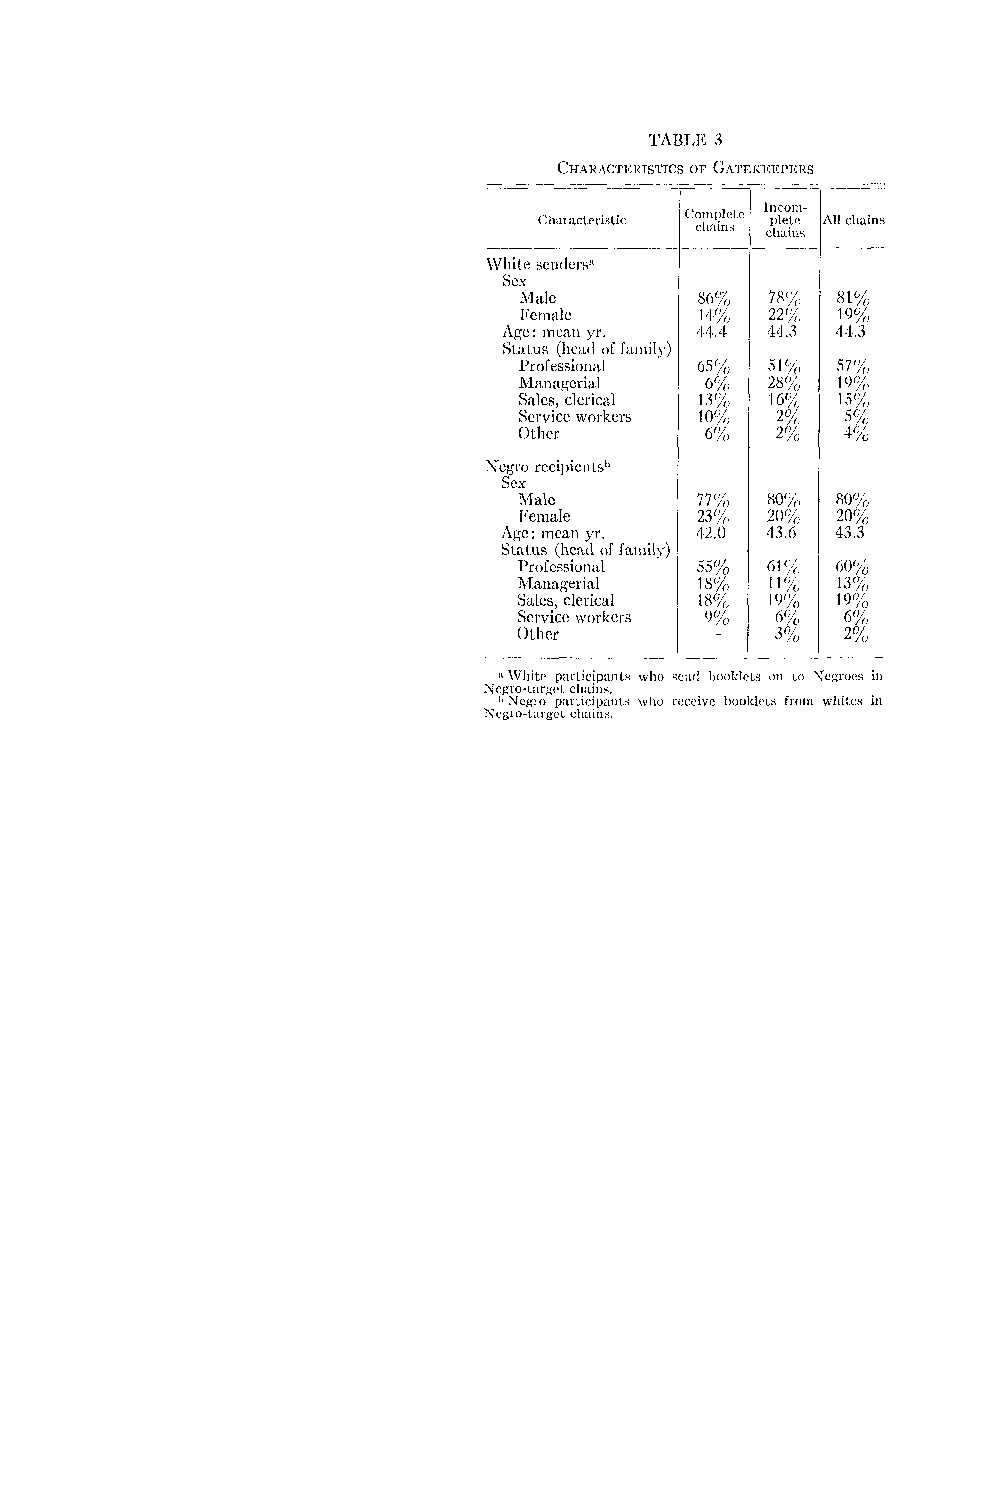
\includegraphics[height=0.6\textheight]{figures/korte_aquaintance_1970_tab3}
\end{center}

\vfill
``Gatekeepers'' of white to ``Negro'' connections were predominately Male professionals\\
In 23 of the 35 successful cross-group chains, the first ``Negro'' was the target\\
Most failed chains (80\%) never crossed the racial boundary\\

\end{frame}
%%%%%%%%%%%%%%%%%%%%%%%%
\begin{frame}

\begin{itemize}
\item Introduction to the connected age
\pause
\item Small world problem shows the scientific arc: idea $\rightarrow$ formal question $\rightarrow$ empirical research $\rightarrow$ critique
\end{itemize}

\end{frame}
%%%%%%%%%%%%%%%%%%%%%%%%%
\begin{frame}

Next class: More on the small world problem and some history

\end{frame}
%%%%%%%%%%%%%%%%%%%%%%%%%



\end{document}
